% Document type
\documentclass[12pt]{article}

% User packages
\usepackage{amsmath}
\usepackage{amssymb}
\usepackage{enumerate}
\usepackage{enumitem}
\usepackage{fancyhdr}
\usepackage{graphicx}
\usepackage{hyperref}
\usepackage[margin = 2.0 cm, includehead, includefoot]{geometry}
\usepackage[table]{xcolor}
\usepackage{verbatim}

% Header and footer settings
\pagestyle{fancy}
\setlength{\headheight}{15 pt}
\lhead{Intel Corporation}
\chead{}
\rhead{Brian Mascitello}
\lfoot{Math Question}
\cfoot{}
\rfoot{Page \thepage}
\renewcommand{\headrulewidth}{0.2 pt}
\renewcommand{\footrulewidth}{0.2 pt}

% Start of the document
\begin{document}

% Titlepage start
\begin{titlepage}
\begin{center}


\includegraphics[scale=0.5]{Intel.png}
\vspace{3 mm}

\huge{Intel Corporation}
\vspace{5 cm}

\huge{Math Question}
\vspace{3 mm}

\huge{December 10, 2015}
\vspace{7 cm}

\huge{Brian Mascitello}

\end{center}
\end{titlepage}
% Titlepage end

%%%%%%%%%%%%%%%%%%%%%%%%%%%%%%%%%%%%%%%%%%%%%%%%%

The problem posed by Hikmat Hajyahya (Mat) is ...
\[ \scalebox{2}{$1 + \sqrt{3}^x = 2^{x}$ , solve for x?} \]

\begin{enumerate}[label=\textbf{\arabic*}.]

\item The first way I attempted solving this was the laziest. Try $x = 0$ ...

$$1 + \sqrt{3}^x = 2^{x}$$

$$1 + \sqrt{3}^0 = 2^{0}$$

$$1 + 1 = 1$$

$$2 = 1$$

This is of course false, thus $x \neq 0$. However it tells us that at $x = 0$ the left side of the equation is greater than the right, but in analyzing the equation we note the right will grow faster than the left side. This is because 1 is constant, thus not dependent on x. $\sqrt{3} \approx 1.732$ and $1.732 < 2$, thus $2^{x}$ increases faster than $1 + \sqrt{3}^x$ as $x$ increases. Try $x = 1$ ...

$$1 + \sqrt{3}^x = 2^{x}$$

$$1 + \sqrt{3}^1 = 2^{1}$$

$$1 + 1.732 = 2$$

$$2.732 = 2$$

Also false, since left side is still larger, try $x = 2$ ...

$$1 + \sqrt{3}^x = 2^{x}$$

$$1 + \sqrt{3}^2 = 2^{2}$$

$$1 + 3 = 4$$

$$4 = 4$$

Since four is indeed equivalent to four, the answer to $1 + \sqrt{3}^x = 2^{x}$ is $x = 2$.

%%%%%%%%%%%%%%%%%%%%%%%%%%%%%%%%%%%%%%%%%%%%%%%%%

\newpage

\item The second way I attempted to solve it, as well as verify the first method, is by graphing it. (Mat didn't want this solution but I'm providing it cause it works.)

Let $y_1 = 1 + \sqrt{3}^x$ and $y_2 = 2^{x}$ , then

\begin{minipage}{.68\linewidth}
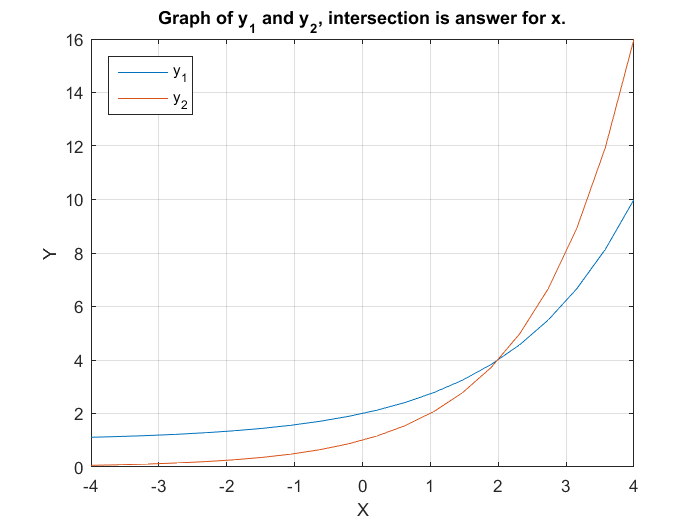
\includegraphics[scale=0.60]{Part2Graph.png}
\end{minipage}
\begin{minipage}{.3\linewidth}
\begin{tabular}{c | c | c}
$x$ & $y_1$ & $y_2$ \\
\hline
4	&	10	&	16 \\
\hline
-4.000	&	1.111	&	0.063	\\
\hline
-3.579	&	1.140	&	0.084	\\
\hline
-3.158	&	1.176	&	0.112	\\
\hline
-2.737	&	1.222	&	0.150	\\
\hline
-2.316	&	1.280	&	0.201	\\
\hline
-1.895	&	1.353	&	0.269	\\
\hline
-1.474	&	1.445	&	0.360	\\
\hline
-1.053	&	1.561	&	0.482	\\
\hline
-0.632	&	1.707	&	0.645	\\
\hline
-0.211	&	1.891	&	0.864	\\
\hline
0.211	&	2.123	&	1.157	\\
\hline
0.632	&	2.415	&	1.549	\\
\hline
1.053	&	2.783	&	2.074	\\
\hline
1.474	&	3.247	&	2.777	\\
\hline
\rowcolor{yellow!50}1.895	&	3.831	&	3.719	\\
\hline
\rowcolor{yellow!50}2.316	&	4.568	&	4.979	\\
\hline
2.737	&	5.497	&	6.666	\\
\hline
3.158	&	6.667	&	8.925	\\
\hline
3.579	&	8.142	&	11.950	\\
\hline
4.000	&	10.000	&	16.000	\\
\end{tabular}

\end{minipage}

\textbf{Matlab raw code for graph:}
\begin{verbatim}
>> x = linspace(-4,4,20);
>> y1 = 1 + sqrt(3).^x;
>> y2 = 2.^x;
>> plot(x, y_1, x, y_2)
>> title('Graph of y_{1} and y_{2}, intersection is answer for x.')
>> xlabel('X')
>> ylabel('Y')
>> legend('y_{1}','y_{2}','Location','northwest')
\end{verbatim}

%%%%%%%%%%%%%%%%%%%%%%%%%%%%%%%%%%%%%%%%%%%%%%%%%

\newpage

\item Another graph, except using a root of the function to find the value of x. (Mat likely didn't want this one either, but it is similar to part four.)

Let $y = 2^{x} - \sqrt{3}^x - 1$ , then 

\begin{minipage}{.68\linewidth}
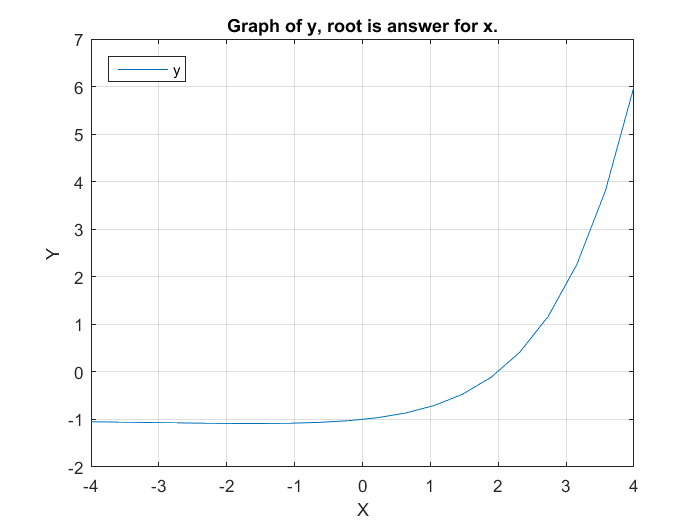
\includegraphics[scale=0.60]{Part3Graph.png}
\end{minipage}
\begin{minipage}{.3\linewidth}
\begin{tabular}{c | c}
$x$ & $y$ \\
\hline
-4.000	&	-1.049	\\
\hline
-3.579	&	-1.056	\\
\hline
-3.158	&	-1.064	\\
\hline
-2.737	&	-1.072	\\
\hline
-2.316	&	-1.079	\\
\hline
-1.895	&	-1.084	\\
\hline
-1.474	&	-1.085	\\
\hline
-1.053	&	-1.079	\\
\hline
-0.632	&	-1.061	\\
\hline
-0.211	&	-1.027	\\
\hline
0.211	&	-0.965	\\
\hline
0.632	&	-0.865	\\
\hline
1.053	&	-0.709	\\
\hline
1.474	&	-0.469	\\
\hline
\rowcolor{yellow!50}1.895	&	-0.113	\\
\hline
\rowcolor{yellow!50}2.316	&	0.411	\\
\hline
2.737	&	1.169	\\
\hline
3.158	&	2.258	\\
\hline
3.579	&	3.808	\\
\hline
4.000	&	6.000	\\

\end{tabular}

\end{minipage}

\textbf{Matlab raw code for graph:}
\begin{verbatim}
>> x = linspace(-4,4,20);
>> y = 2.^x - sqrt(3).^x - 1;
>> plot(x, y)
>> title('Graph of y, root is answer for x.')
>> grid on
>> xlabel('X')
>> ylabel('Y')
>> legend('y','Location','northwest')
\end{verbatim}

%%%%%%%%%%%%%%%%%%%%%%%%%%%%%%%%%%%%%%%%%%%%%%%%%

\newpage

\item This is the toughest way to solve for x that I can think of in this case, and it does not require graphs so hopefully this is what Mat really wanted.

Let $y = 2^{x} - \sqrt{3}^x - 1$ , then find the derivative of $y$.

$$y = 2^{x} - 3^{x/2} - 1$$

$$\dfrac{d}{dx}y = \dfrac{d}{dx}(2^{x} - 3^{x/2} - 1)$$

$$y' = \dfrac{d}{dx}(2^{x}) \dfrac{d}{dx}(- 3^{x/2}) \dfrac{d}{dx}(- 1)$$

$$y' = \dfrac{d}{dx}(2^{x}) - \dfrac{d}{dx}(3^{x/2})$$

$$y' = 2^{x}ln(2) - \dfrac{d}{dx}(3^{x/2})$$

$$\boxed{y' = 2^{x}ln(2) - \dfrac{3^{x/2}ln(3)}{2}}$$

$ln(2) \approx 0.693147$ and $ln(3) \approx 1.098612$

\textbf{\textit{Newton's Method}}
\hspace{3 mm} If $x_n$ is an approximation a solution of  and if  the next approximation is given by,

$$x_{n+1} = x_n - \dfrac{f(x_n)}{f'(x_n)}$$

\newpage

\textbf{Mat's Problem.py raw code:}
\begin{verbatim}
# Created by Brian Mascitello to calculate a specific
# polynomial given to me by Mat at Intel.

def matsproblem(x0):
    """ function matsproblem(x0) finds a root of the nonlinear
        function specified by f and fprime. y = 2 ** x - 3 ** (x / 2) - 1;
        yprime = 0.693147 * (2 ** x) - (1.098612 * 3 ** (x / 2)) / 2; Result
        x is the root. """

    epsilon = 2.2204*10**-16
    """ governs precision of convergence
        where 2.2204*10**-16 = machine epsilion in python """
    
    x = x0
    xprevious = 0
    k = 0

    while abs(float(2 ** x - 3 ** (x / 2) - 1)) > epsilon*abs(float(2 
    ** x0 - 3 ** (x0 / 2) - 1)) and k < 20:
        k = k+1
        xprevious = x
        x = float(x) - (float(2 ** x - 3 ** (x / 2) - 1)/float(0.693147 
        * (2 ** x) - (1.098612 * 3 ** (x / 2)) / 2))
        change = abs(float(x - xprevious))
        residual = 2 ** x - 3 ** (x / 2) - 1
        print("Iteration: %d, Root: %f, Change: %f, Residual: %f" % 
        (k,x,change,residual))
    
    print("Root at",x,"\n")

    return float(x)

print("y = 2 ** x - 3 ** (x / 2) - 1")
print("yprime = 0.693147 * (2 ** x) - (1.098612 * 3 ** (x / 2)) / 2")
print("Machine epsilon set as: 2.2204*10^-16")
x0 = float(input("Please enter your guess of the root: "))
matsproblem(x0)
\end{verbatim}

\newpage

\textbf{Mat's Problem.py output:}
\begin{verbatim}
y = 2 ** x - 3 ** (x / 2) - 1
yprime = 0.693147 * (2 ** x) - (1.098612 * 3 ** (x / 2)) / 2
Machine epsilon set as: 2.2204*10^-16
Please enter your guess of the root: 0
Iteration: 1, Root: 6.952121, Change: 6.952121, Residual: 77.270274
Iteration: 2, Root: 5.681332, Change: 1.270789, Residual: 27.651539
Iteration: 3, Root: 4.485320, Change: 1.196012, Residual: 9.648804
Iteration: 4, Root: 3.421652, Change: 1.063668, Residual: 3.165227
Iteration: 5, Root: 2.595079, Change: 0.826573, Residual: 0.882313
Iteration: 6, Root: 2.131456, Change: 0.463623, Residual: 0.156953
Iteration: 7, Root: 2.007459, Change: 0.123998, Residual: 0.008417
Iteration: 8, Root: 2.000025, Change: 0.007433, Residual: 0.000028
Iteration: 9, Root: 2.000000, Change: 0.000025, Residual: 0.000000
Iteration: 10, Root: 2.000000, Change: 0.000000, Residual: -0.000000
Iteration: 11, Root: 2.000000, Change: 0.000000, Residual: 0.000000
Root at 2.0
\end{verbatim}

This program applies Netwon's Method to solve for x. It requires taking the derivative of the original equation and carefully implementing it to get a precise answer. You could calculate this by hand but everyone loved python so much I thought I would re-purpose newtoncube.py for this occasion.

%%%%%%%%%%%%%%%%%%%%%%%%%%%%%%%%%%%%%%%%%%%%%%%%%

\end{enumerate}

\end{document}